\documentclass{beamer}
\usetheme{Warsaw}
\setbeamertemplate{caption}[numbered]
\setbeamertemplate{navigation symbols}{}%remove navigation symbols

\usepackage{polski}
\usepackage[utf8]{inputenc}
\usepackage{array}
\usepackage{hyperref}
\usepackage{listings}

\title{Optymalizacja struktury sieci drogowej}
\author{Michał Siatkowski} 
\institute{Promotor: dr hab. inż. Aneta Poniszewska - Marańda \\
		Kopromotor: mgr inż. Łukasz Chomątek \\
		\vspace*{20px}
		Politechnika Łódzka}
\date{Łódź, FTIMS, Informatyka 2014/2015}

\begin{document}

\maketitle

\section{Wstep}
\subsection{Problematyka i zakres pracy}
\begin{frame}{Problematyka optymalizacji ruchu drogowego} 

\begin{figure}[b]
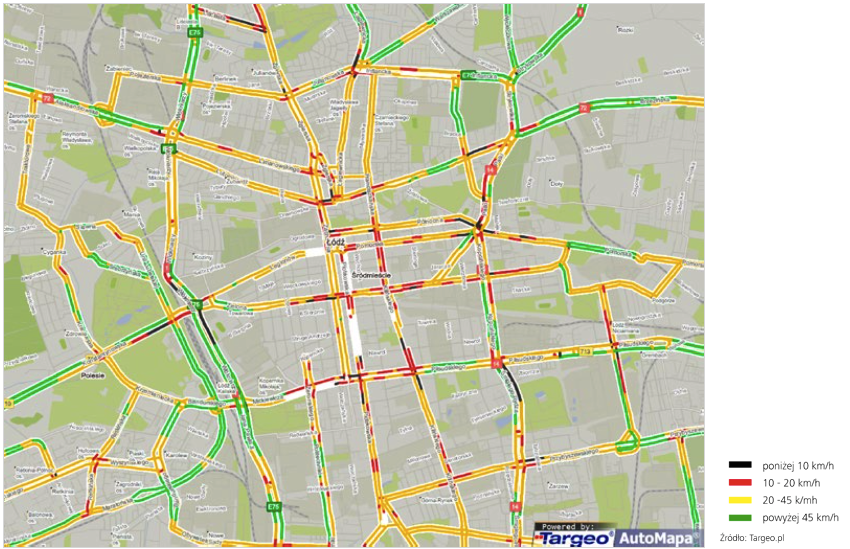
\includegraphics[width=0.85\textwidth]{img/lodz}
\caption{Łódź - szczyt poranny, średnie prędkości.}
\end{figure}

\end{frame}


\subsection{Cele pracy}
\begin{frame}{Cele pracy} 

Celami pracy są:
\begin{enumerate}

\item Zdefiniowanie problematyki optymalizacji struktury sieci drogowej.
\item Stworzenie aplikacji optymalizującej tę strukturę.
\item Analiza i ocena efektywności zastosowanych rozwiązań.

\end{enumerate}

\end{frame}

\section{Optymalizacja struktury sieci drogowej}

\subsection{Podstawowe definicje}
\begin{frame}{Podstawowe definicje} 

\newtheorem{mydef1}{Sieć drogowa}
\begin{mydef1}
	\begin{figure}[h!]
	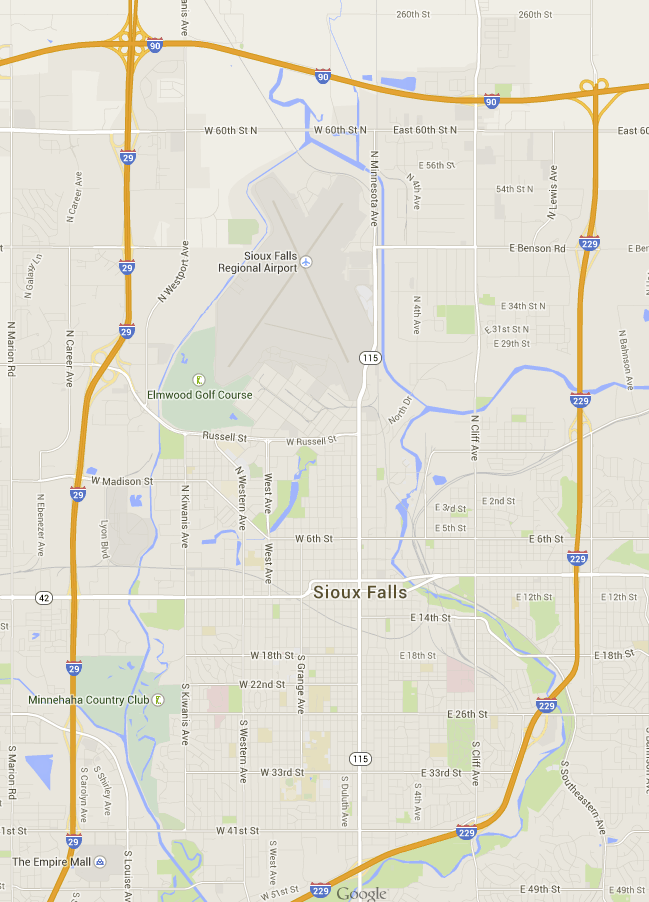
\includegraphics[width=0.30\textwidth]{img/siec}
	\caption{Fragment sieci drogowej w Sioux Falls, Południowa Dakota.} 
	\end{figure}
\end{mydef1}

\end{frame}

\begin{frame}{Podstawowe definicje} 

\newtheorem{mydef2}{Sieć drogowa w postaci grafu}
\begin{mydef2}
	\begin{figure}[h!]
	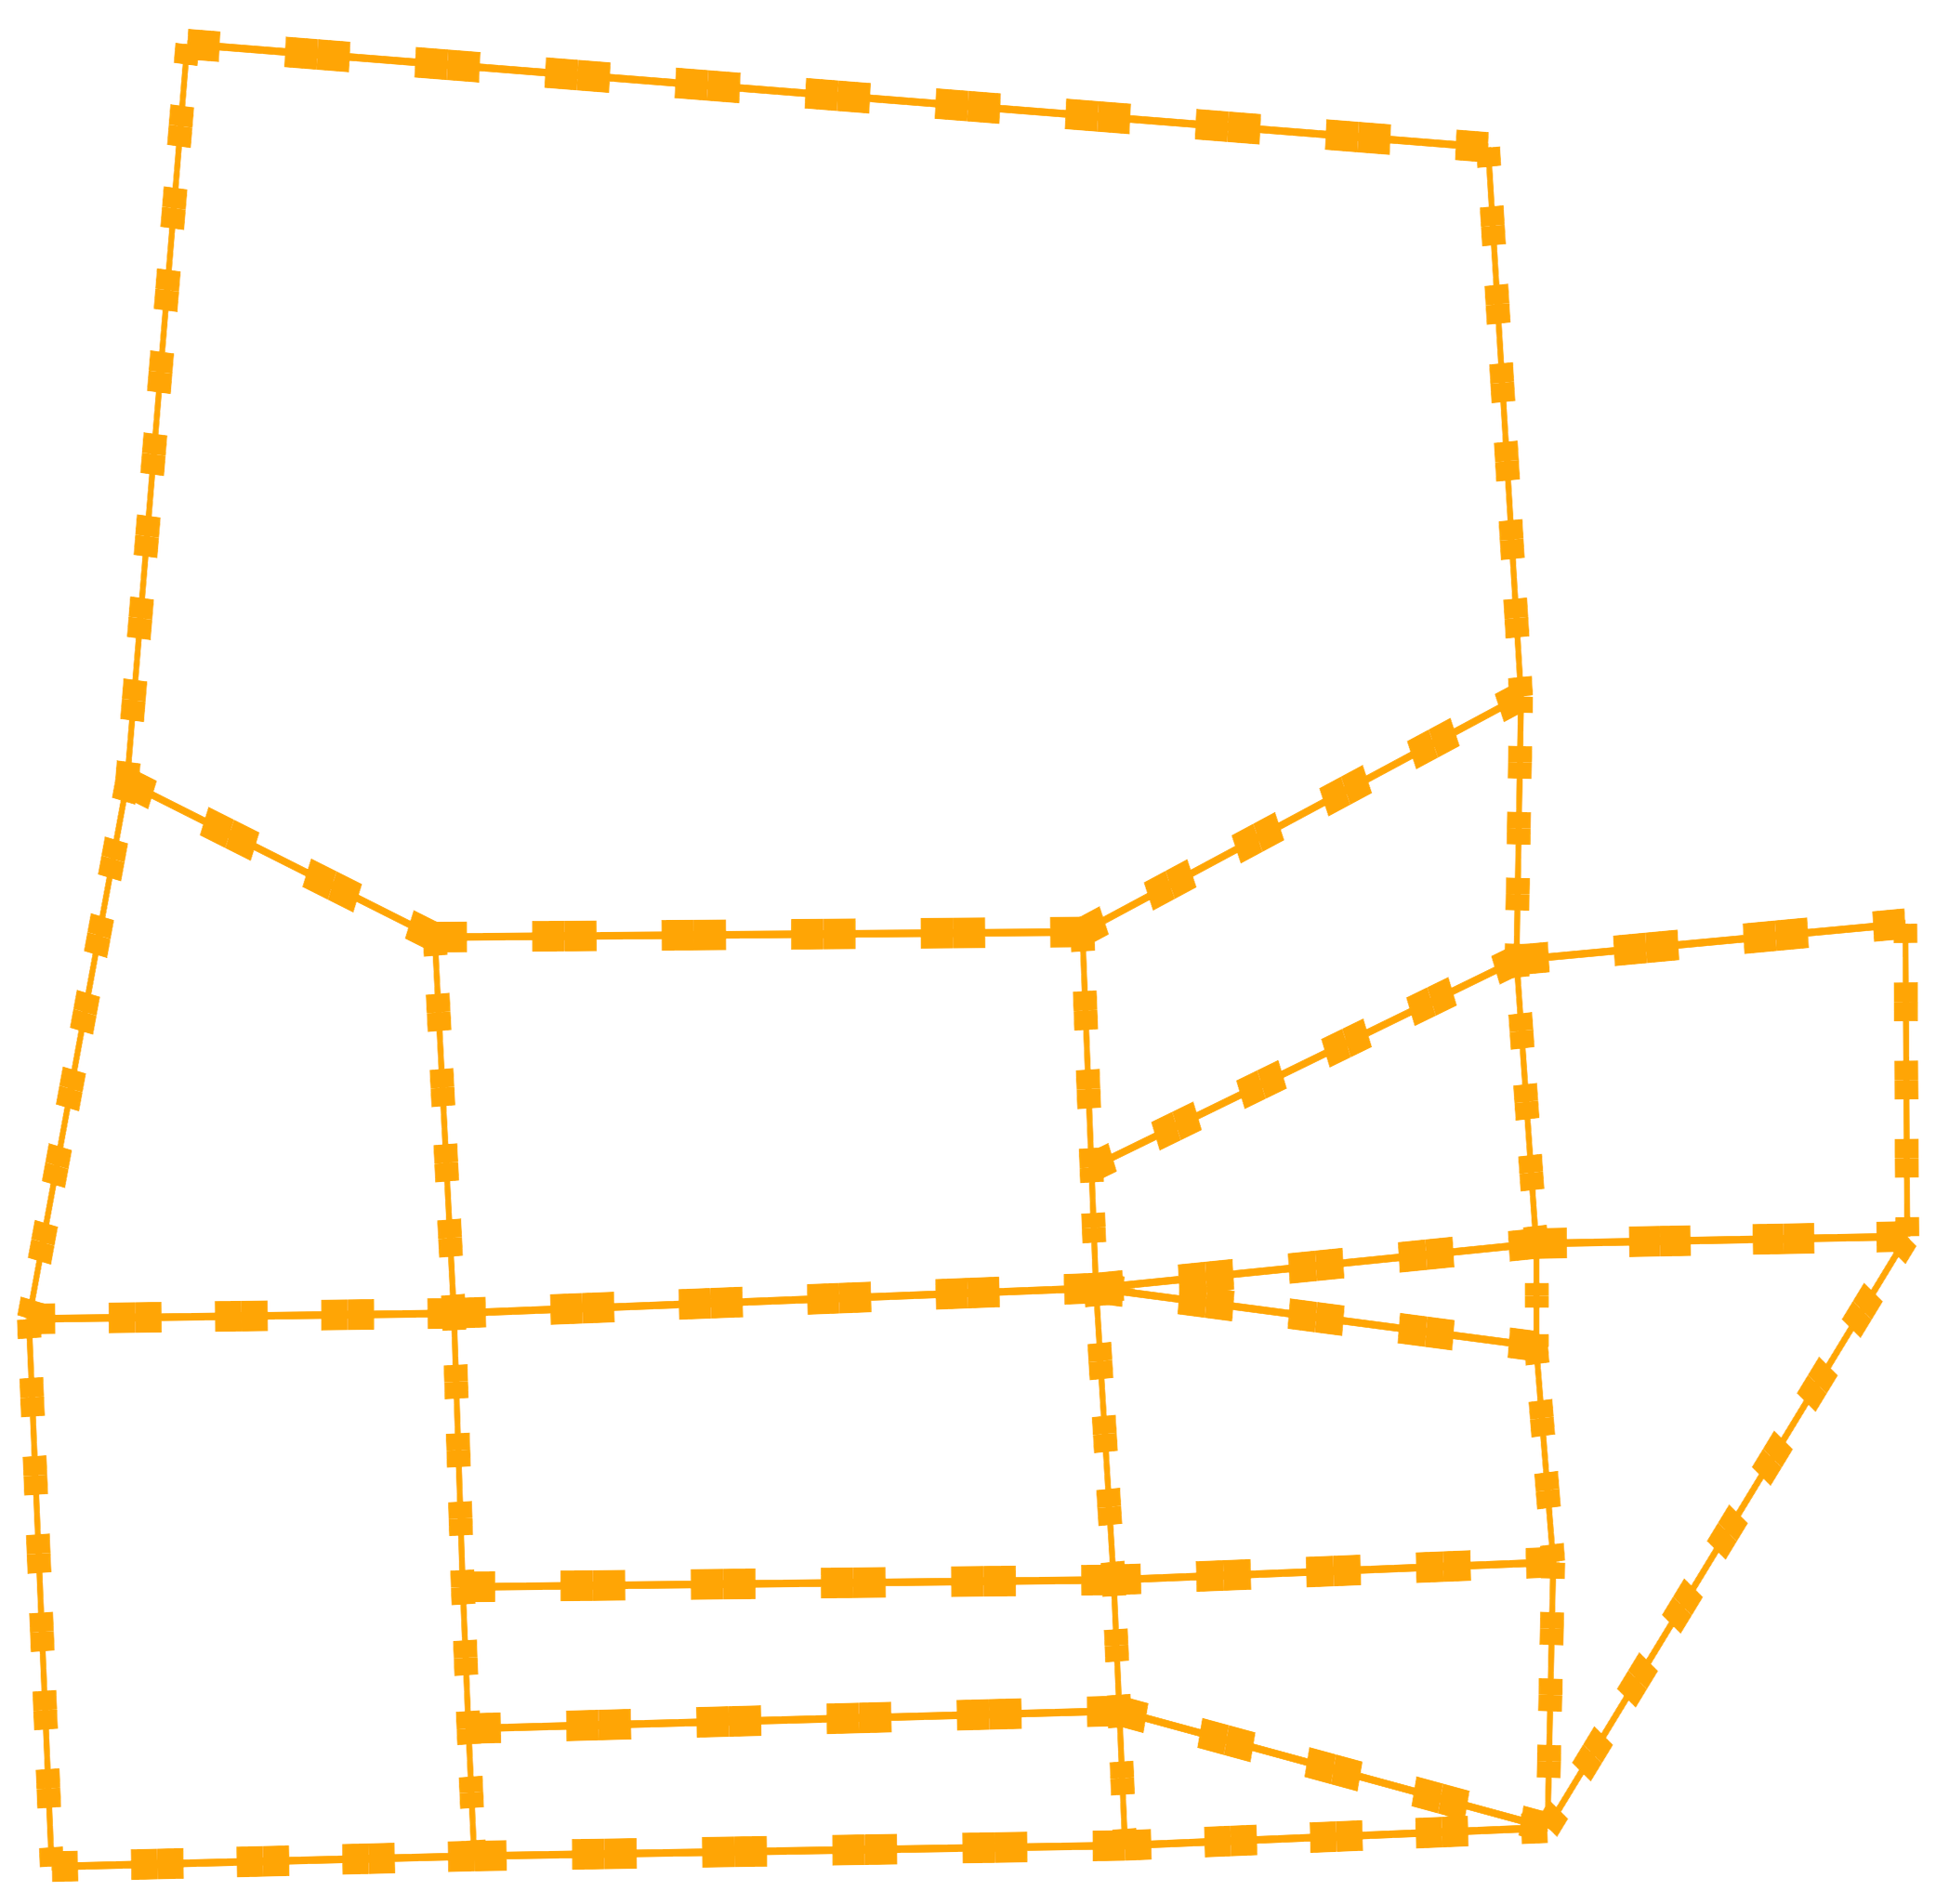
\includegraphics[width=0.45\textwidth]{img/graf}
	\caption{Siec drogowa miasta Sioux Falls w postaci grafu.} 
	\end{figure}
\end{mydef2}
\end{frame}


\subsection{Paradoks Braessa }
\begin{frame}{Paradoks Braessa}

\centering
\begin{minipage}{.48\textwidth}
\begin{figure}[h!]
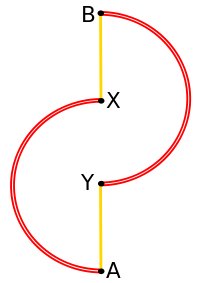
\includegraphics[width=0.7\textwidth]{img/braess1}
\caption{Wyjściowy układ drogowy}
\end{figure}
\end{minipage}\hfill
\begin{minipage}{.48\textwidth}

Autostrady:\\
AX, $t_{AX}(p) =  50 + p$ min\\
YB, $t_{YB}(p) =  50 + p$ min\\

Drogi lokalne:\\
AY, $t_{AY}(p) =  10p$ min\\
XB, $t_{XB}(p) =  10p$ min\\
\\
Aut jest 6000 i wszystkie mają za zadanie przejechać trasę z A do B.

\end{minipage}\hfill

\end{frame}


\begin{frame}{Równowaga Nasha} 

Równowaga Nasha to taka sytuacja, w której każdy z samochodów spowoduje wydłużenie swojego czasu jazdy, zmieniając decyzję co do wyboru trasy przy niezmienionych decyzjach pozostałych aut.
\newline\newline
Jeśli p i q to liczby aut w tysiącach pokonujących odpowiednio trasy AXB i AYB, otrzymujmy równania:

\begin{center}
$p+q = 6 $\\
$t_{AX}(p)+t_{XB}(p) = t_{AY}(q) + t_{YB}(q)$\\
$50+p+10p = 10q+50+q$
\end{center}
rozwiązaniem jest $p=q=3$.\\
Przy tej gęstości ruchu pokonanie obu dostępnych tras zabiera $50+3+30=83$ minuty.
\end{frame}

\begin{frame}{Uzupełniony układ drogowy} 

\centering
\begin{minipage}{.48\textwidth}
\begin{figure}[h!]
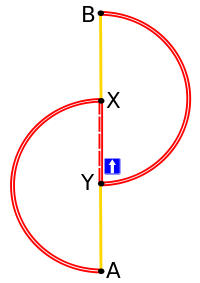
\includegraphics[width=0.7\textwidth]{img/braess2}
\caption{Uzupełniony układ drogowy}
\end{figure}
\end{minipage}\hfill
\begin{minipage}{.48\textwidth}
Do wyjściowego układu drogowego dodana zostaje autostrada:\\

YX, $t_{YX}(p) =  10 + p$ min\\

Aut jest nadal 6000 i wszystkie mają za zadanie przejechać trasę z A do B.

\end{minipage}\hfill
\end{frame}

\begin{frame}{Równowaga Nasha dla uzupełnionego układu} 

Jeśli p, q i r to liczby aut w tysiącach pokonujących odpowiednio trasy AXB, AYB i AYXB, otrzymujmy równania:

\begin{center}
$p+q+r = 6 $\\
$t_{AX}(p)+t_{XB}(p+r) = t_{AY}(q+r) + t_{YB}(q) = t_{AY}(q+r)+t_{YX}(r)+t_{XB}(p+r)$
\newline\\
$50+p+10(p+r) = 10(q+r)+50+q = 10(q+r)+ 10 + r + 10(p+r)$
\end{center}
rozwiązaniem jest $p=q=r=2$.\\
Czas przejazdu każdej z tych dróg wynosi wówczas $50+2+10(2+2)=92$ minuty.
\end{frame}


\subsection{Symulator transportu}
\begin{frame}{Symulator transportu} 

\begin{figure}[b]

\includegraphics[width=0.30\textwidth]{img/matsim}
\caption{Logo symulatora transportu MATSim}
\end{figure}

\begin{itemize}
\item{Dostarcza symulację zachowań mobilnych opartych na agentach.} 
\item{Zapewnia szybkość i~stabilność działania.} 
\item{Przedstawia analizę dostarczanych wyników.} 
\item{Pozwala na podejście modułowe.} 
\item{Został stworzony w~ramach licencji otwartego oprogramowania.} 
\end{itemize}

\end{frame}

\begin{frame}{Klasyczny algorytm genetyczny} 

\centering
\begin{minipage}[b]{.48\textwidth}
\begin{figure}[]
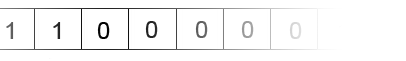
\includegraphics[width=\textwidth]{img/bool}
\caption{Fragment sieci w postaci tablicy binarnej }
\end{figure}
\end{minipage}\hfill
\begin{minipage}[b]{.48\textwidth}
\begin{figure}[]
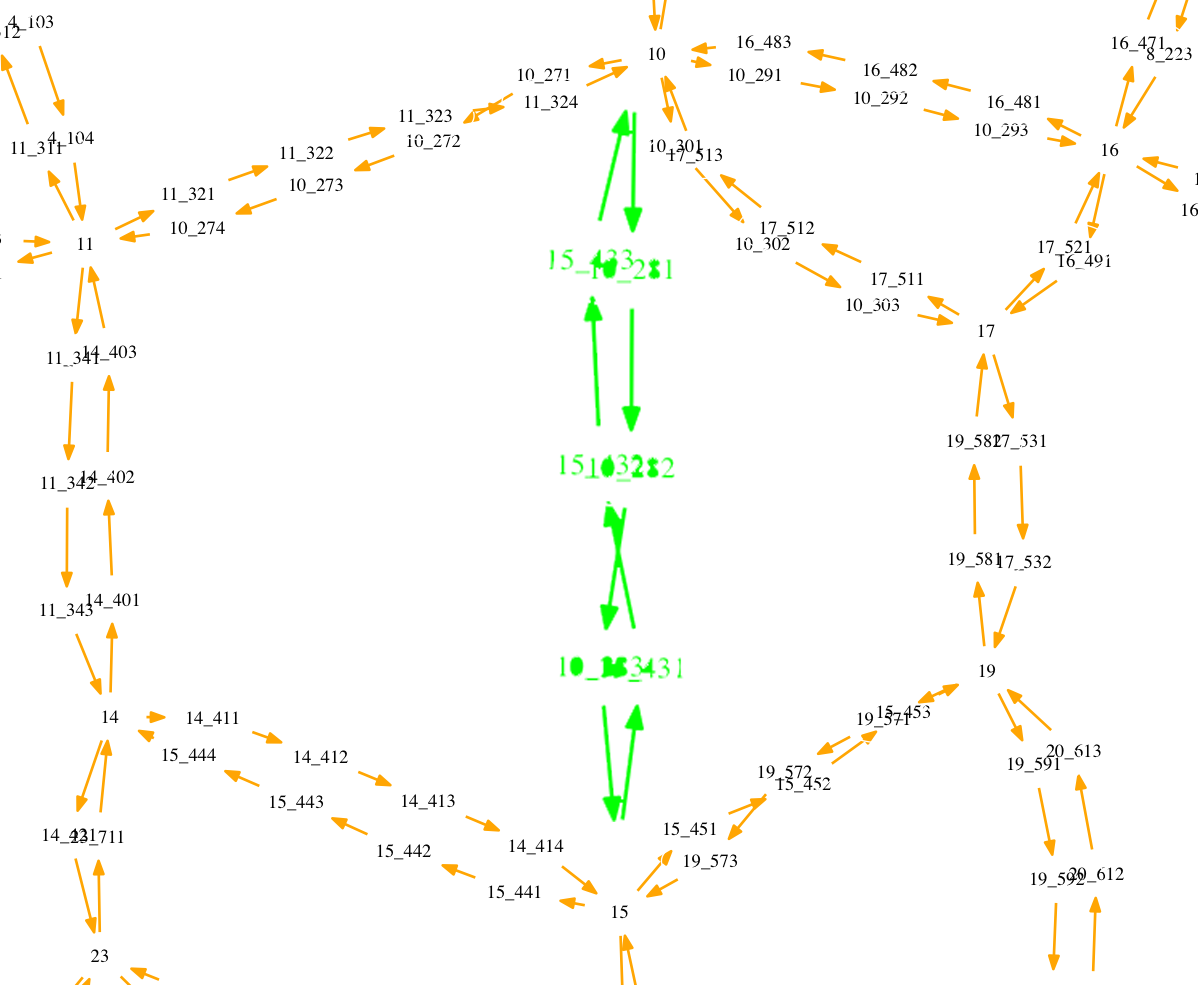
\includegraphics[width=\textwidth]{img/bool-efect}
\caption{Fragment sieci w postaci grafu}
\end{figure}
\end{minipage}\hfill
\end{frame}


\section{Podsumowanie}
\subsection{Prezentacja wyników}
\begin{frame}{Zamykane obszary} 
\begin{figure}[b]
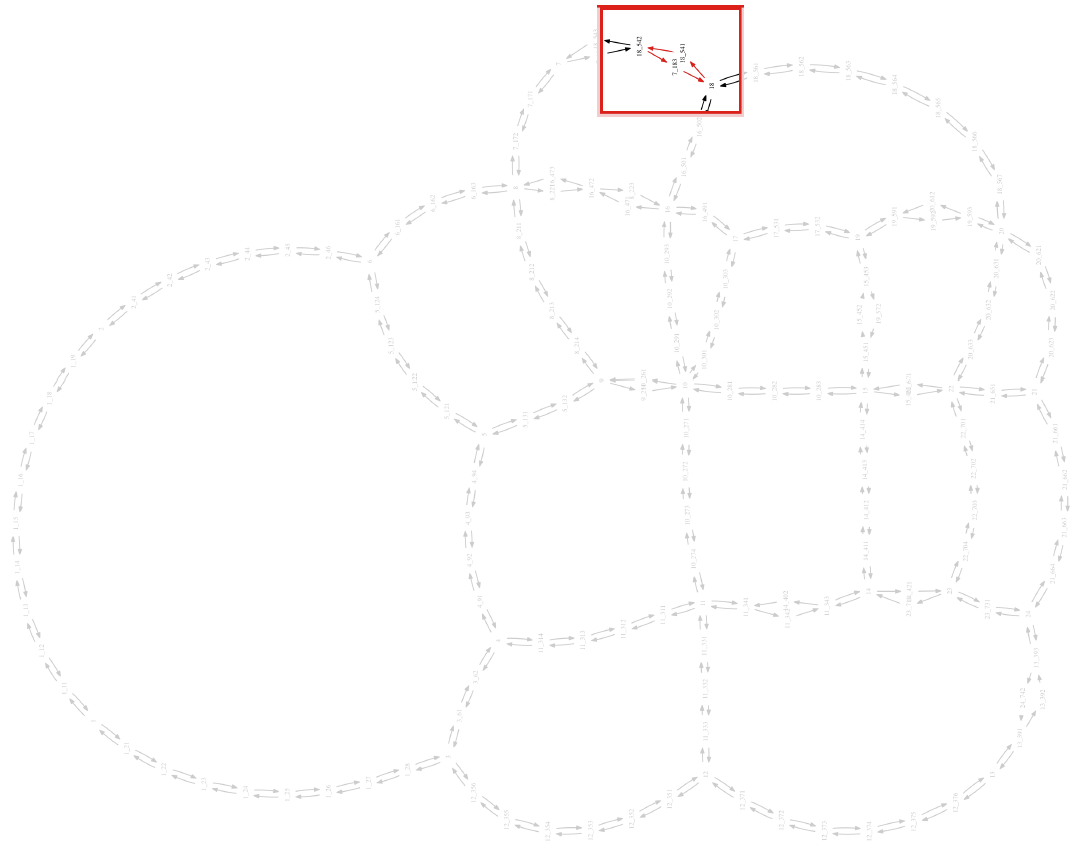
\includegraphics[width=0.666\textwidth]{img/wspolne3}
\caption{Graf z zaznaczonym zamkniętym obszarem wspólnie dla wszystkich wyników.}
\end{figure}
\end{frame}

\begin{frame}{Zamykane obszary} 
\begin{figure}[b]
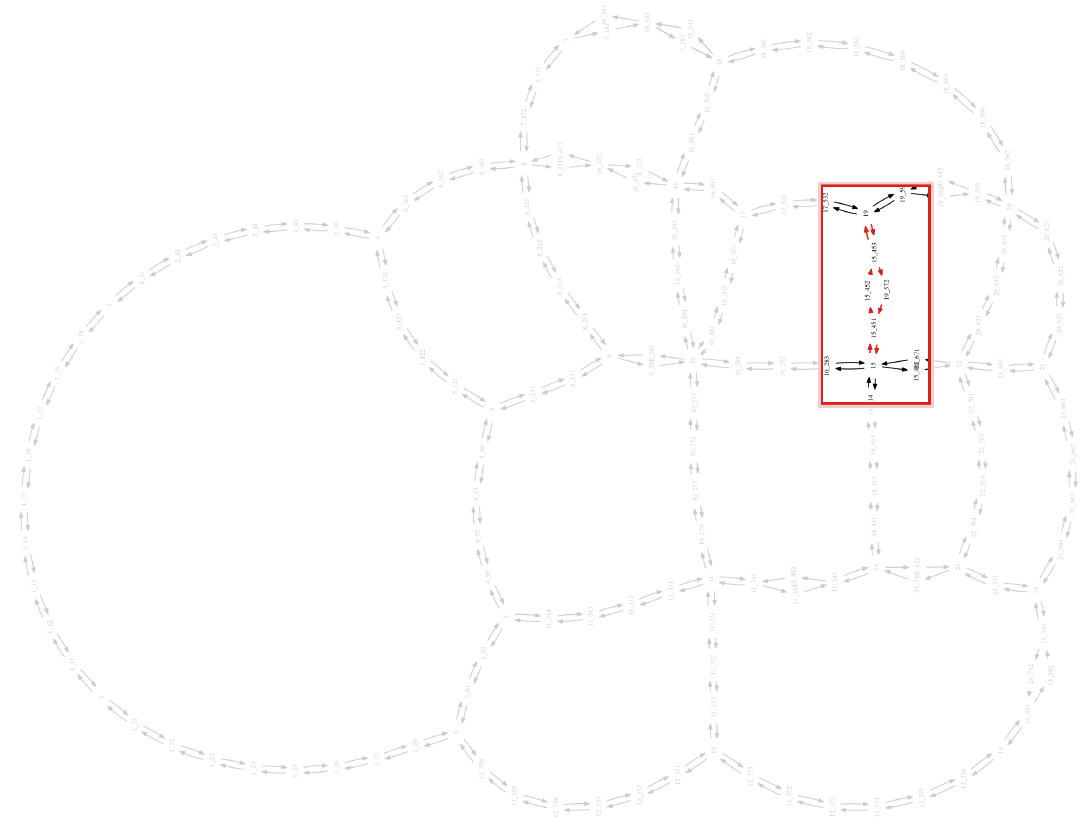
\includegraphics[width=0.666\textwidth]{img/wspolne1}
\caption{Graf z zaznaczonym zamkniętym obszarem wspólnie dla wyników o ID: 5, 7, 9, 10, 11, 12, 13, 14, 16.}
\end{figure}
\end{frame}

\begin{frame}{Zamykane obszary} 
\begin{figure}[b]
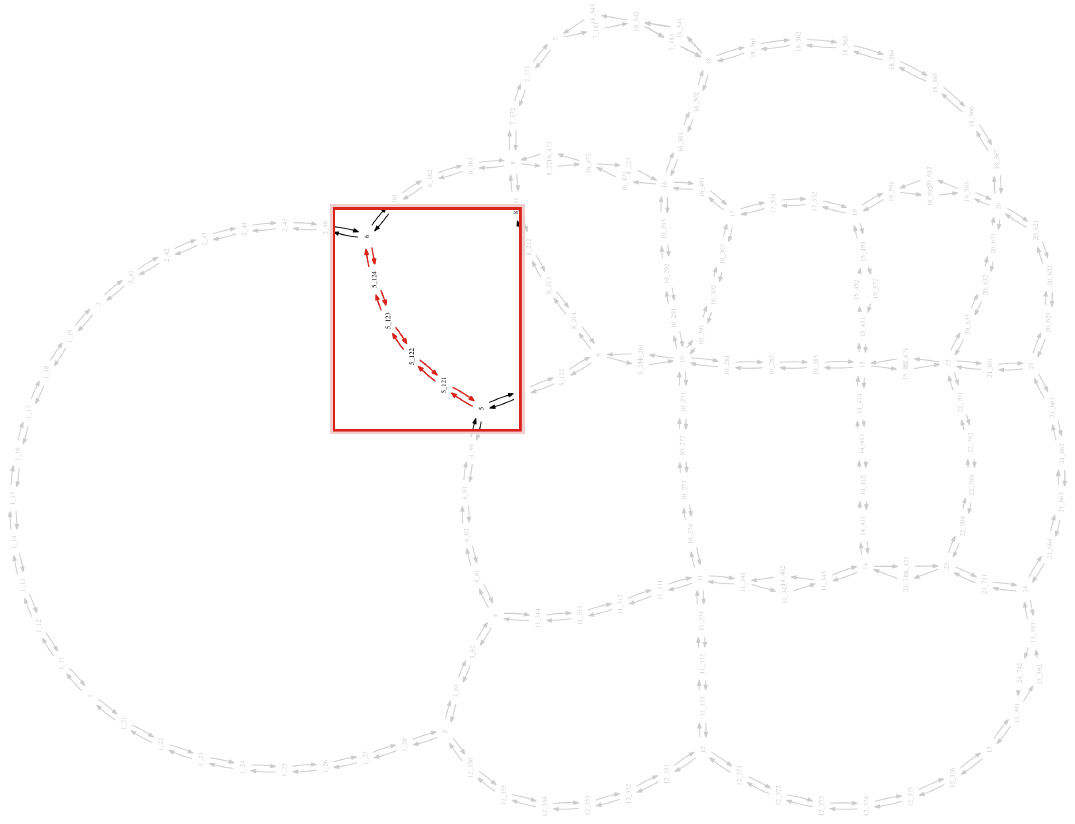
\includegraphics[width=0.666\textwidth]{img/wspolne4}
\caption{Graf z zaznaczonym zamkniętym obszarem wspólnie dla wyników o ID: 2, 4, 6, 8, 12.}
\end{figure}
\end{frame}

\begin{frame}{Zamykane obszary} 
\begin{figure}[b]
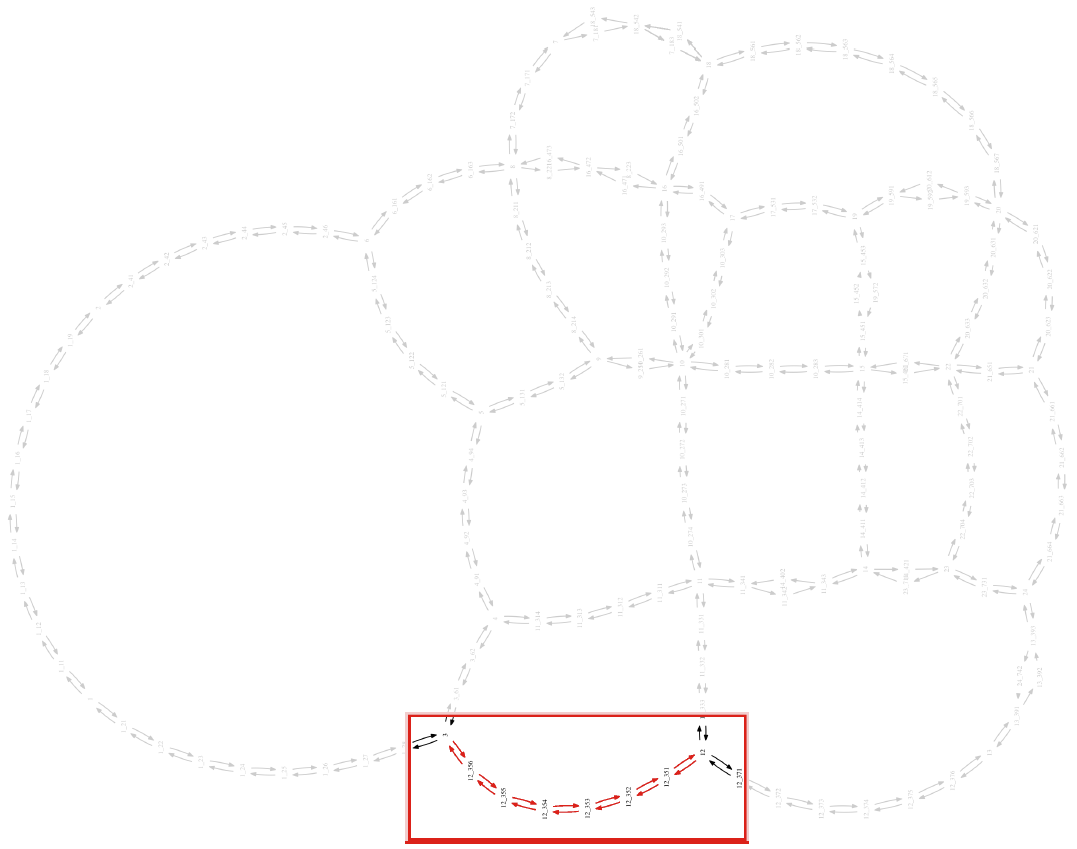
\includegraphics[width=0.666\textwidth]{img/wspolne2}
\caption{Graf z zaznaczonym zamkniętym obszarem wspólnie dla wyników o ID: 3, 8, 15.}
\end{figure}
\end{frame}

\subsection{Porównanie wyników}
\begin{frame}{Wyniki optymalizacji sieci} 
\begin{figure}[b]
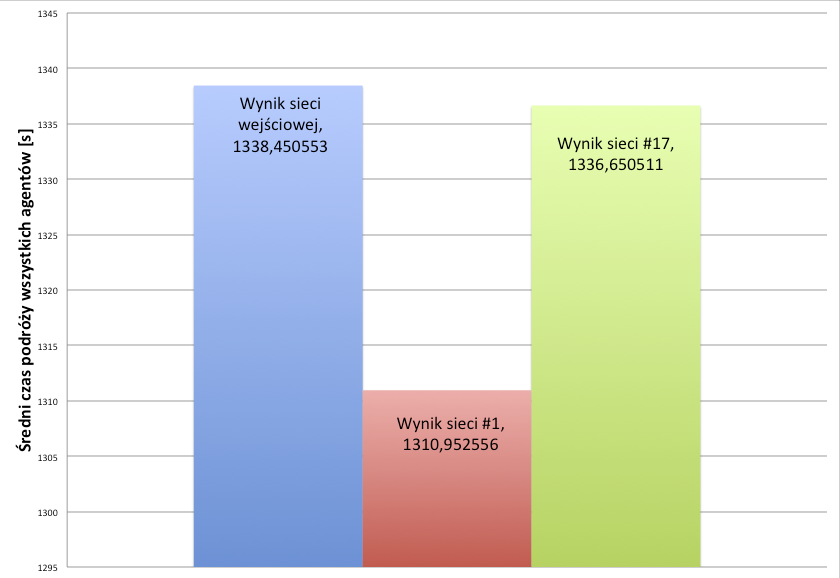
\includegraphics[width=0.8\textwidth]{img/wyniki}
\caption{Wykres porównujący wyniki optymalizacji.}
\end{figure}
\end{frame}


\end{document}